\documentclass[a4paper]{article}
\usepackage{vntex}
%\usepackage[english,vietnam]{babel}
%\usepackage[utf8]{vietnam}

%\usepackage[utf8]{inputenc}
%\usepackage[francais]{babel}
\usepackage{a4wide,amssymb,epsfig,latexsym,multicol,array,hhline,fancyhdr}

\usepackage{float}
\usepackage{amsmath}
\usepackage{lastpage}
\usepackage[lined,boxed,commentsnumbered]{algorithm2e}
\usepackage{enumerate}
\usepackage{color}
\usepackage{graphicx}							% Standard graphics package
\usepackage{array}
\usepackage{tabularx, caption}
\usepackage{multirow}
\usepackage{multicol}
\usepackage{rotating}
\usepackage{geometry}
\usepackage{xcolor}
\usepackage{longtable}
\usepackage{setspace}
\usepackage{epsfig}
\usepackage{tikz}
\usepackage{cite}
\usetikzlibrary{arrows,snakes,backgrounds}
\usepackage{hyperref}
\hypersetup{urlcolor=blue,linkcolor=black,citecolor=black,colorlinks=true} 
%\usepackage{pstcol} 								% PSTricks with the standard color package

%\usepackage{fancyhdr}
\setlength{\headheight}{40pt}
\pagestyle{fancy}
\fancyhead{} % clear all header fields
\fancyhead[L]{
 \begin{tabular}{rl}
    \begin{picture}(25,15)(0,0)
    \put(0,-8){
\includegraphics[width=8mm, height=8mm]{hcmut.png}}
    %\put(0,-8){\epsfig{width=10mm,figure=hcmut.eps}}
   \end{picture}&
	%
\includegraphics[width=8mm, height=8mm]{hcmut.png} & %
	\begin{tabular}{l}
		\textbf{\bf \ttfamily Trường Đại Học Bách Khoa Tp.Hồ Chí Minh}\\
		\textbf{\bf \ttfamily Khoa Khoa Học và Kỹ Thuật Máy Tính}
	\end{tabular} 	
 \end{tabular}
}
\fancyhead[R]{
	\begin{tabular}{l}
		\tiny \bf \\
		\tiny \bf 
	\end{tabular}  }
\fancyfoot{} % clear all footer fields
\fancyfoot[L]{\scriptsize \ttfamily Bài tập lớn môn Lập trình hướng đối tượng
}
\fancyfoot[R]{\scriptsize \ttfamily Trang {\thepage}/\pageref{LastPage}}
\renewcommand{\headrulewidth}{0.3pt}
\renewcommand{\footrulewidth}{0.3pt}


%%%
\setcounter{secnumdepth}{4}
\setcounter{tocdepth}{3}
\makeatletter
\newcounter {subsubsubsection}[subsubsection]
\renewcommand\thesubsubsubsection{\thesubsubsection .\@alph\c@subsubsubsection}
\newcommand\subsubsubsection{\@startsection{subsubsubsection}{4}{\z@}%
                                     {-3.25ex\@plus -1ex \@minus -.2ex}%
                                     {1.5ex \@plus .2ex}%
                                     {\normalfont\normalsize\bfseries}}
\newcommand*\l@subsubsubsection{\@dottedtocline{3}{10.0em}{4.1em}}
\newcommand*{\subsubsubsectionmark}[1]{}
\makeatother


\begin{document}
\begin{titlepage}
\begin{center}
ĐẠI HỌC QUỐC GIA THÀNH PHỐ HỒ CHÍ MINH \\
TRƯỜNG ĐẠI HỌC BÁCH KHOA \\
KHOA KHOA HỌC - KỸ THUẬT MÁY TÍNH 
\end{center}

\vspace{1cm}

\begin{figure}[h!]
\begin{center}

\includegraphics[width=3cm]{hcmut.png}
\end{center}
\end{figure}

\vspace{1cm}


\begin{center}
\begin{tabular}{c}
\multicolumn{1}{l}{\color{blue}{{\textbf{{\Large LẬP TRÌNH HƯỚNG ĐỐI TƯỢNG}}}}}\\
~~\\
\hline
\\
\multicolumn{1}{l}{\color{blue}{\textbf{{\Large BÀI TẬP LỚN}}}}\\
\\
\color{blue}{\textbf{{\large ỨNG DỤNG TRÊN ĐIỆN THOẠI VỚI C\#}}}\\
\\
\hline
\end{tabular}
\end{center}

\vspace{3cm}


\begin{table}[h]
\hspace{5 cm}
\begin{tabular}{rll}
 GV: & Mai Đức Trung\\
\hline
  SV: & Nguyễn Huỳnh Minh & 1813085 \\
    & Võ Minh Long & 1812951 \\
     & Đoàn Ngọc Thịnh  & 1810542 \\
     
\end{tabular}
\end{table}

\vspace{2cm}
\begin{center}
{\footnotesize TP. HỒ CHÍ MINH, THÁNG 11/2019}
\end{center}
\end{titlepage}

\newpage
\tableofcontents
\newpage
\section{Giới thiệu}
\subsection{Giới thiệu về sản phẩm}
\hspace*{1 cm}Đây là sản phầm từ \textit{bài tập lớn} của môn \textbf{lập trình hướng đối tượng}, được thực hiện bởi nhóm \textit{Blue Stream}. Với hi vọng sẽ tạo ra một sản phẩm có ích và đáp ứng yêu cầu môn học, cả nhóm đã lên ý tưởng về việc tạo ra 1 ứng dụng chạy trên nền tảng điện thoại, cụ thể là \textit{Android}, vì tính phổ biến của nền tảng này. Cuối cùng, cả nhóm đã thống nhất sẽ làm 1 ứng dụng liên quan đến chính bản thân mỗi sinh viên, để hỗ trợ tốt hơn trong việc sắp xếp thời gian, cũng như học tập. Mà cụ thể ở đây là mong muốn tạo ứng dụng có khả năng xem thời khóa biểu, lịch thi, thi thử.\\
\hspace*{1 cm} Sản phầm này chỉ có sinh viên \textit{trường Đại học Bách Khoa TP.Hồ Chí Minh} mới có thể sử dụng được. Vì còn hạn chế về kĩ năng, kinh nghiệm, thời gian,... nên ứng dụng có những vấn đề chưa thật sự tốt, và như ý muốn.\\
\hspace*{1 cm}Ứng dụng được viết bằng ngôn ngữ lập trình \textit{C\#} với framework chính là \textit{Xamarin}, ngoài ra còn sử dụng \textit{SQLite}, \textit{Firebase} để lưu trữ dữ liệu,...
\subsection{Xamarin}
\subsubsection{Xamarin là gì?}
\begin{itemize}
    \item  Xamarin là một framework của \textit{Mỉcrosoft}, dùng để xây dựng ứng dụng trên điện thoại đa nền tảng. Với công nghệ đa nền tảng(cross-platform), Xamarin sẽ giúp nhà phát triển chỉ với cùng một mã nguồn có thể tạo ra được cả 3 ứng dụng chạy trên 3 nền tảng khác nhau: Android, IOS, Windows Phone. Và có thể chia sẻ mã nguồn qua nhiều nền tảng như : Windows, macOS, Linux.
\item Xamarin sử dụng ngôn ngữ \textit{C\#} và các thư viện \textit{native} được gói trong các gói \textit{.NET} cho phép phát triển đa nền tảng. 
\item Xamarin hiện nay hoạt động trên Xamarin IDE(MAC),  Microsoft Visual Studio(Windows) hay Rider IDE(Linux).
\end{itemize}
\subsubsection{Ưu điểm}
\begin{itemize}
    \item Đa nền tảng - đặc điểm quan trọng của Xamarin: người lập trình có thể viết chung một mã nguồn cho nhiều nền tảng khác nhau.
    \item Hỗ trợ \textit{UI Native} trải nghiệm tốt hơn các framework cross-platform khác.
    \item Lập trình với \textit{C\#} hiệu quả và đỡ tốn sức hơn so với \textit{native}.
    \item Hiệu năng của ứng dụng lập trình bằng Xamarin giờ đây đã được cải thiện rất nhiều, gần ngang ngửa với ứng dụng được xây dựng bằng \textit{native code}.
    \item Có thể dễ dàng chia sẽ mã nguồn do ứng dụng được xây dựng cùng một ngôn ngữ, API, cấu trúc dữ liệu, giúp tiết kiệm thời gian đáng kể.
\end{itemize}
\subsubsection{Hạn chế}
\begin{itemize}
    \item Khả năng cập nhật lên nền tảng mới còn chậm.
    \item Mang khuyết điểm của \textit{AOT Compiler (Ahead-Of-Time)}: các đoạn code không được gọn gàng, dung lượng ứng dụng sẽ lớn hơn so với ứng dụng \textit{native code}. Điều này dấn đến khả năng phát triển ứng dụng trở nên khó khăn hơn.
\end{itemize}
\newpage
\section{Phân tích ứng dụng}
\begin{figure}[htp]
    \centering
    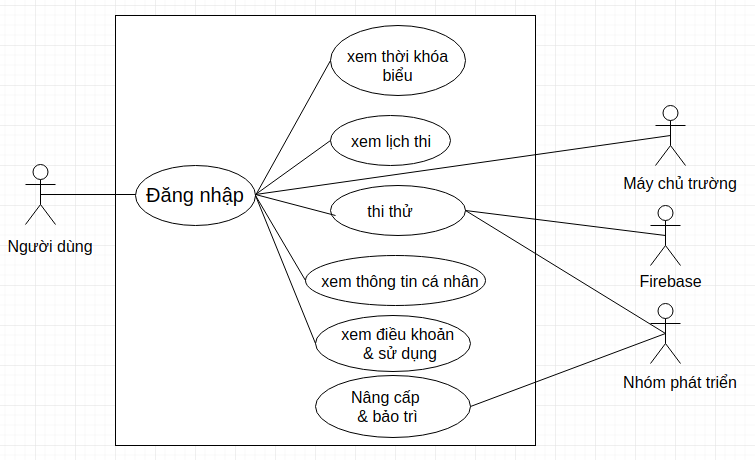
\includegraphics[scale = .35]{usecase.png}
    \caption{Bản vẽ Use Case của ứng dụng}
    \label{fig:usecase}
\end{figure}
Quan sát bản vẽ Use Case hình \ref{fig:usecase}, ta có thấy ứng dụng gồm có 6 khối chức năng chính mà người dùng có thể tương tác: đăng nhập, thời khóa biểu, lịch thi, thi thử, thông tin cá nhân, điều khoản & sử dụng. Chúng ta sẽ đi cụ thể vào từng khối.
\subsection{Yêu cầu}
\begin{itemize}
    \item Viết bằng ngôn ngữ lập trình \textit{C\#}
    \item Ứng dụng chỉ chạy trên nền tảng \textbf{Android phiên bản 5.0} trở lên.
    \item Phải có tài khoản \textbf{MyBK} của \textit{trường Đại học Bách Khoa TP.Hồ Chí Minh}
    \item Chạy tốt nhất trên các thiết bị có tỉ lệ màn hình $16:9$, cụ thể  là màn hình có độ phân giải $1280$x$720$
\end{itemize}
\subsection{Đăng nhập}
\hspace*{.5 cm}Đây là khối chức năng đầu tiên, cũng là bước quan trọng. Vì nếu không qua được khối này, thì người dùng không thể sử dụng các chức năng tiếp theo. Lưu đồ của khối này ở hình \ref{fig:login}. \\
\begin{figure}[H]
    \centering
    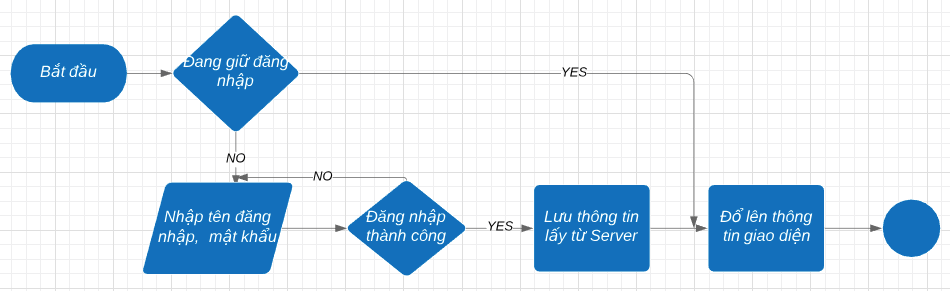
\includegraphics[scale=.4]{loginflow.png}
    \caption{Lưu đồ khối đăng nhập}
    \label{fig:login}
\end{figure}
\hspace*{.5 cm}Khi mới mở ứng dụng, đầu tiên sẽ kiểm tra nếu đã đăng nhập trước đó, và còn đang giữ trạng thái này, thì chỉ cần hiển thị lại thông tin đã được lưu lên giao diện. Ngược lại, thì người dùng cần cung cấp \textit{tên đăng nhập} và \textit{mật khẩu}. Nếu đăng nhập thành công, thì thông tin lấy được từ máy chủ gồm có: thời khóa biểu, lịch thi, thông tin cá nhân, dữ liệu câu hỏi sẽ được lưu lại. Rồi hiển thị các thông tin này lên giao diện, còn không thì phải nhập lại thông tin đăng nhập.
\subsection {Thời khóa biểu}
\hspace*{0.5 cm}Sau khi đăng nhập thành công, giao diện hiện ra đầu tiên là \textit{thời khóa biểu} của tuần học tương ứng. Dữ liệu được truy vấn từ \textit{database} lưu trên thiết bị. Lưu đồ cụ thể như hình \ref{fig:scheduler}.\\
\begin{figure}[h!]
    \centering
    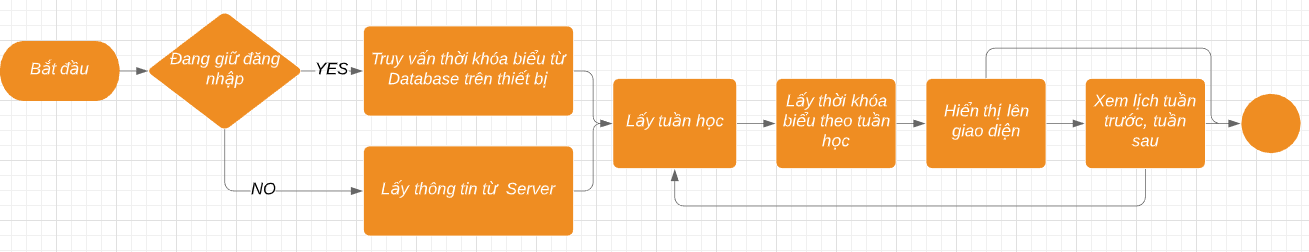
\includegraphics[scale=.4]{schedulerflow.png}
    \caption{Lưu đồ khối thời khóa biểu}
    \label{fig:scheduler}
\end{figure}\\
\hspace*{0.5 cm}Thời khóa biểu gồm có lịch học của nhiều tuần, nhưng ứng dụng chỉ hiển thị lịch học của tuần hiện tại theo từng ngày. Bên cạnh đó, người dùng cũng có thể xem lịch học của tuần trước hoặc tuần tiếp theo.
\subsection{Lịch thi}
\hspace*{.5 cm} Khối này gần giống với khối \textit{thời khóa biểu}. Lưu đồ cụ thể như hình dưới:
\begin{figure}[H]
    \centering
    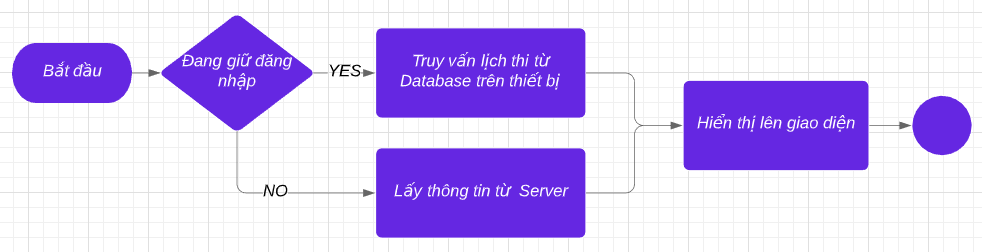
\includegraphics[scale=.4]{exam.png}
    \caption{Lưu đồ khối lịch thi}
\end{figure}\\
\hspace*{0.5 cm}Chức năng khối này đơn giản là lấy lại thông tin được lưu trên thiết bị, sau đó hiển thị lịch thi theo \textit{giữa kì} hay \textit{cuối kì}, và sắp xếp theo thứ tự diễn ra.
\subsection{Thi thử}
\hspace*{.5 cm} Đây là khối chức năng quan trọng, cũng là khá phức tạp hơn khi so với 3 khối trước. Lưu đồ cụ thể ở hình \ref{test}.
\begin{figure}[h!]
    \centering
    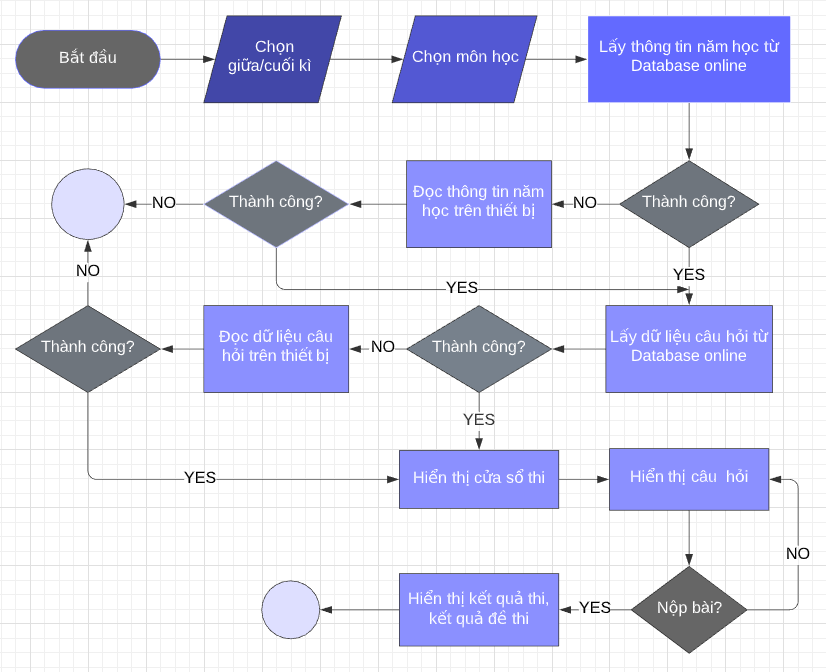
\includegraphics[scale=.4]{test.png}
    \caption{Lưu đồ khối thi thử}
    \label{test}
\end{figure}\\
\hspace*{0.5 cm}Ban đầu, người dùng cần chọn muốn thi thử giữa kì, hay cuối kì. Sau đó, sẽ hiện ra danh sách các môn học đang học trong kì đó, chọn tiếp 1 môn. Sau khi chọn xong, sẽ gửi yêu cầu lấy dữ liệu đến \textit{database online}, hoặc là \textit{dữ liệu lưu trên thiết bị}. Nếu quá trình này thành công, sẽ mở ra cửa sổ thi, hiển thị các câu hỏi, ngược lại thì sẽ thông báo \textit{'không có dữ liệu'}. Người dùng có thể nộp bài bất cứ lúc nào muốn để xem kết quả thi, và đáp án đề thi.
\subsection{Thông tin cá nhân}
\hspace*{0.5cm} Đây là khối chức năng bổ sung, giúp người dùng có thể quản lí, kiểm tra thông tin tài khoản cá nhân. Dữ liệu được trích xuất trực tiếp từ server và được lưu vào thiết bị di động thông qua SQLite. Lưu đồ cụ thể ở hình \ref{infoSV}.
\begin{figure}[h!]
    \centering
    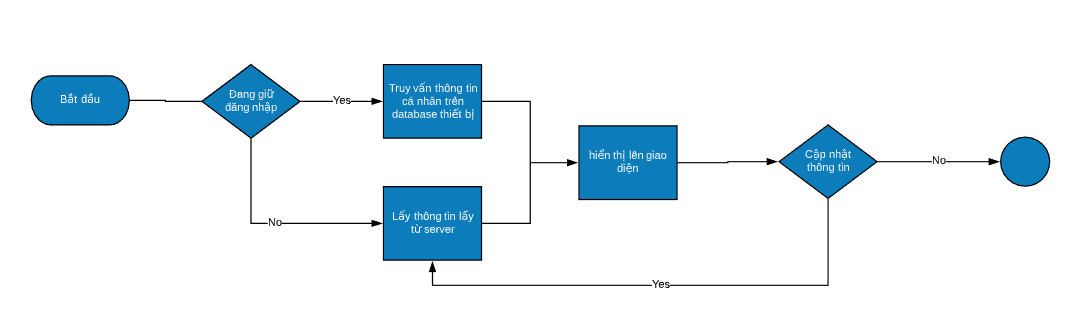
\includegraphics[scale=.4]{thong_tin_ca_nhan.PNG}
    \caption{Lưu đồ thông tin cá nhân}
    \label{infoSV}
\end{figure}\\

\subsection{Điều khoản}
    Hiển thị những điều khoản mà team cam kết đối với người dùng về dữ liệu thông tin cá nhân, đồng thời những yêu cầu của team đối với người dùng nhằm bảo đảm những quyền lợi của team. Điều khoản được viết dạng file text và được đọc khi app chạy. Lưu đồ cụ thể ở hình \ref{dieukhoan}.
\begin{figure}[h!]
    \centering
    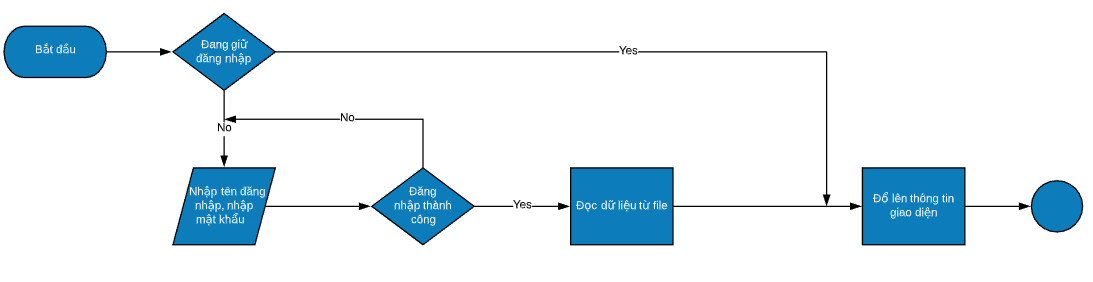
\includegraphics[scale=.4]{dieukhoan.PNG}
    \caption{Lưu đồ khối điều khoản}
    \label{dieukhoan}
\end{figure}\\
\section{Thiết kế ứng dụng}
\subsection{Lược đồ lớp khối đăng nhập}
Lược đồ lớp khối đăng nhập cụ thể ở hình \ref{fig:uml_login}.
\begin{figure}[H]
    \centering
    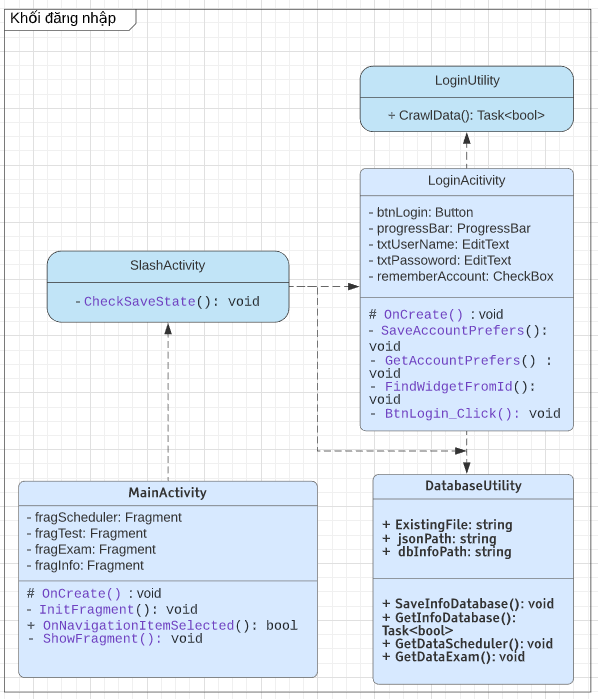
\includegraphics[scale = .5]{uml_login.png}
    \caption{Bản vẽ lớp khối đăng nhập}
    \label{fig:uml_login}
\end{figure}
\subsection{Lược đồ lớp khối thời khóa biểu}
Lược đồ lớp của khối thời khóa biểu ở hình \ref{fig:uml_scheduler}. 
\begin{figure}[H]
    \centering
    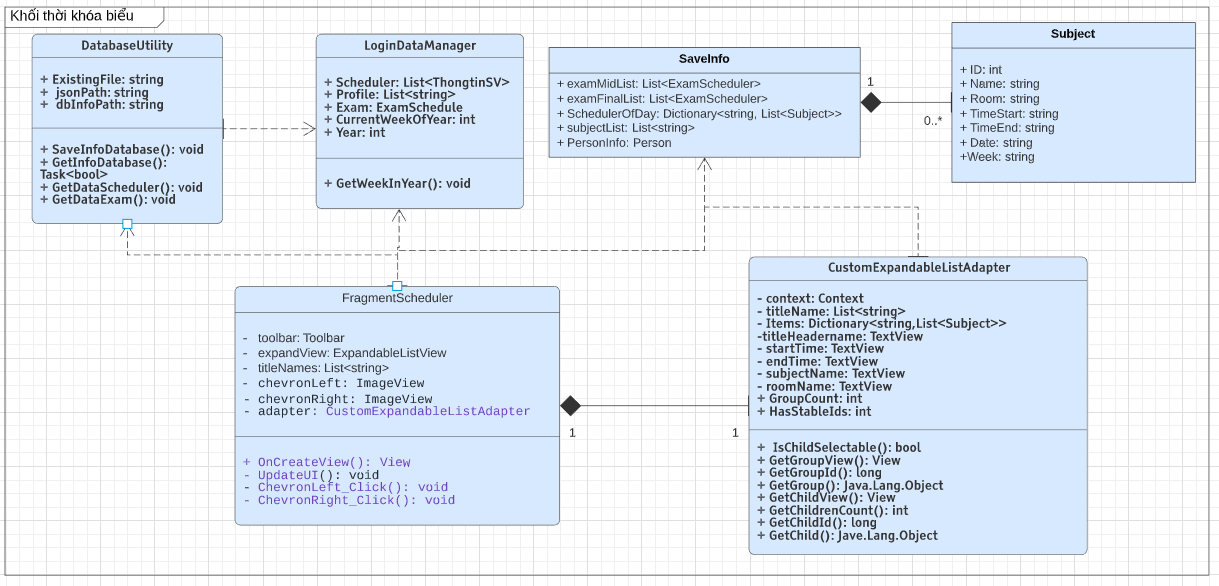
\includegraphics[scale = .4]{uml_scheduler.png}
    \caption{Bản vẽ lớp khối thời khóa biểu}
    \label{fig:uml_scheduler}
\end{figure}
\subsection{Lược đồ lớp khối lịch thi}
Lược đồ lớp của khối lịch thi ở hình \ref{fig:uml_exam}. 
\begin{figure}[H]
    \centering
    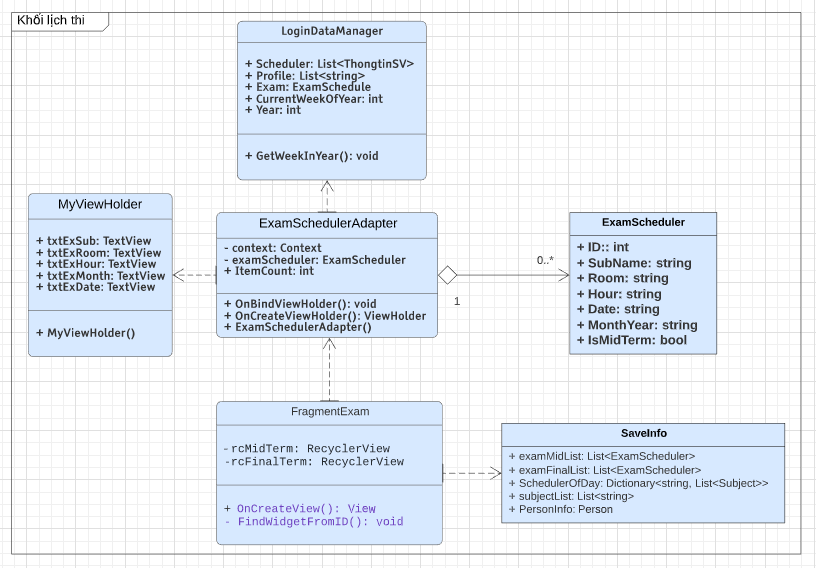
\includegraphics[scale = .5]{uml_exam.png}
    \caption{Bản vẽ lớp khối lịch thi}
    \label{fig:uml_exam}
\end{figure}
\subsection{Lược đồ lớp thi thử}
Lược đồ lớp của khối thi thử được chia làm 2 khối nhỏ hơn: khối chọn môn thi và khối thi. Lược đồ của khối chọn môn thi ở hình \ref{fig:uml_choose}.
\begin{figure}[H]
    \centering
    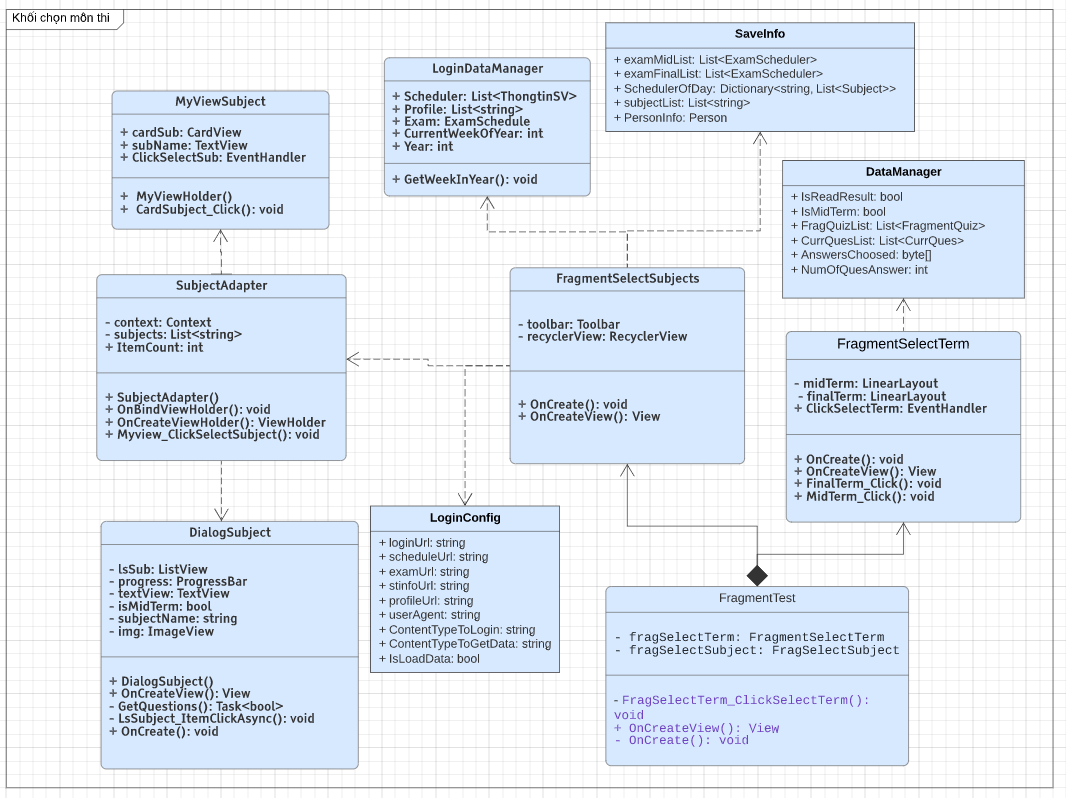
\includegraphics[scale=.4]{uml_choose.png}
    \caption{Bản vẽ lớp khối chọn môn thi}
    \label{fig:uml_choose}
\end{figure}
Lược đồ của khối thi ở hình \ref{fig:uml_test}.Hai khối chọn môn thi và khối thi sẽ tương tác với nhau qua class \textit{DialogSubject}, tạo ra khối lớn hơn là khối thi thử.
\begin{figure}[H]
    \centering
    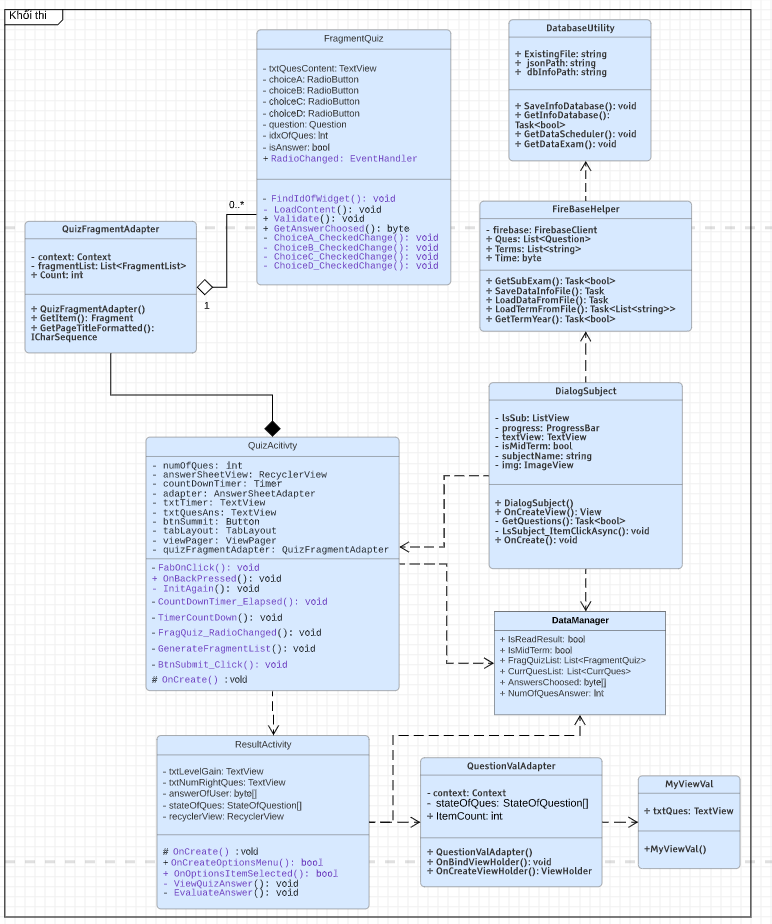
\includegraphics[scale = .5]{uml_test.png}
    \caption{Bản vẽ lớp khối thi}
    \label{fig:uml_test}
\end{figure}

\subsection{Lược đồ lớp khối thông tin cá nhân}
Lược đồ lớp của khối thông tin cá nhân cụ thể ở hình \ref{fig:uml_info}.
\begin{figure}[h]
    \centering
    \includegraphics{}
    \caption{Bản vẽ lớp khối thông tin cá nhân}
    \label{fig:uml_info}
\end{figure}
\subsection{Lược đồ lớp tổng thể}
Lược đồ lớp của ứng dụng sau khi ghép các khối nhỏ hơn ở hình \ref{fig:uml_all}.
\begin{figure}[H]
    \centering
    \includegraphics{}
    \caption{Bản vẽ lớp của ứng dụng}
    \label{fig:uml_all}
\end{figure}
\section{Hướng dẫn về ứng dụng}
Khi mới khởi động ứng dụng lên, giao diện cửa sổ hiện ra  sẽ là màn hình đăng nhập nếu là lần đầu đăng nhập (hoặc đăng xuất). Nếu còn giữ trạng thái đăng nhập thì sẽ bỏ qua bước này.
\begin{figure}[H]
    \centering
    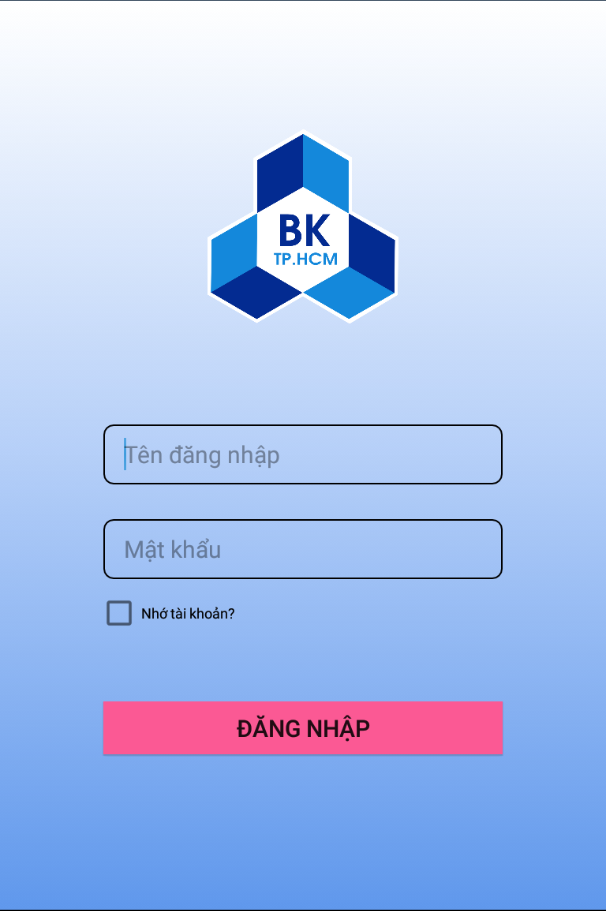
\includegraphics[scale=.3]{login.png}
    \caption{Giao diện màn hình đăng nhập}
\end{figure}
Chúng ta cần có tài khoản \textbf{MyBK} của trường \textit{đại học Bách Khoa TP.Hồ Chí Minh} để có thể xác thực thành công. Sau khi qua được bước đăng nhập (nếu có), giao diện tiếp theo là thông tin về thời khóa biểu.
\begin{figure}[H]
    \centering
    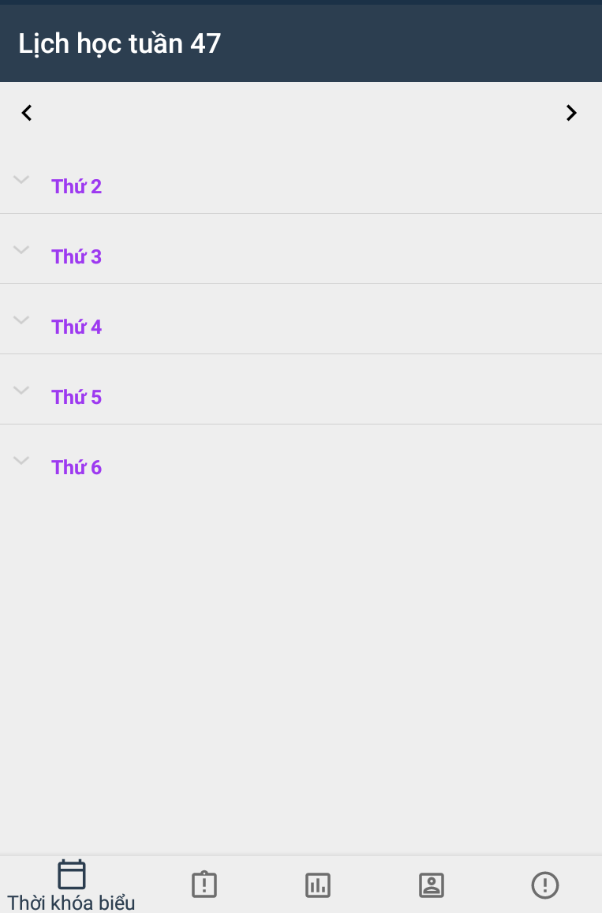
\includegraphics[scale=.3]{scheduler_ui.png}
    \caption{Giao diện màn hình thời khóa biểu}
\end{figure}
Chúng ta có thể xem lịch học của tuần đang diễn ra, hoặc xem lịch học của tuần trước đó/tiếp theo. Ở dưới có 5 nút điều hướng có các chức năng khác nhau. Khi nhấn nút kế bên, sẽ là lịch thi.
\begin{figure}[H]
    \centering
    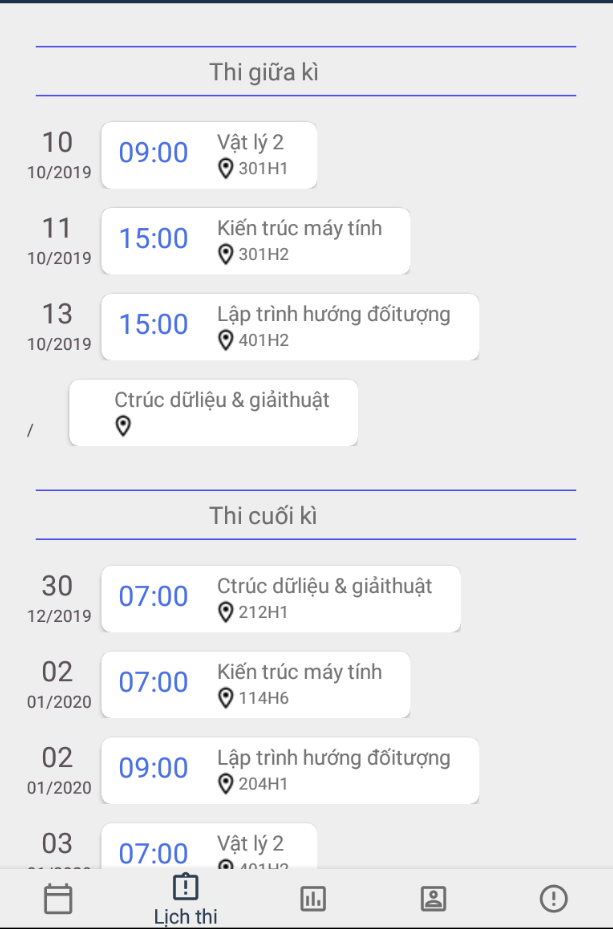
\includegraphics[scale=.3]{exam_ui.png}
    \caption{Giao diện màn hình lịch thi}
\end{figure}
Nhấn tiếp nút kế bên, sẽ là chức năng thi thử. Đầu tiên, chúng ta cần chọn là muốn thi thử giữa kì hay cuối kì.
\begin{figure}[H]
    \centering
    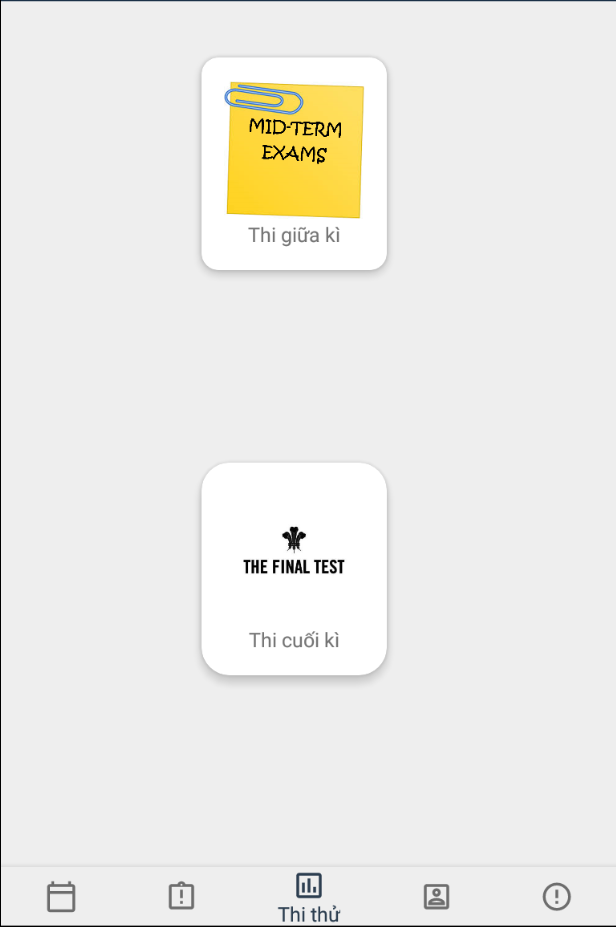
\includegraphics[scale=.3]{test_ui.png}
    \caption{Giao diện màn hình chọn giữa/cuối kì}
\end{figure}
Sau đó, màn hình hiện ra danh sách các môn đang học ở kì này. Và chúng ta cần chọn một môn để thi thử. Vì mỗi người sẽ có các môn học khác nhau, nên hình \ref{fig:sel_sub} chỉ là hình ảnh minh họa.
\begin{figure}[H]
    \centering
    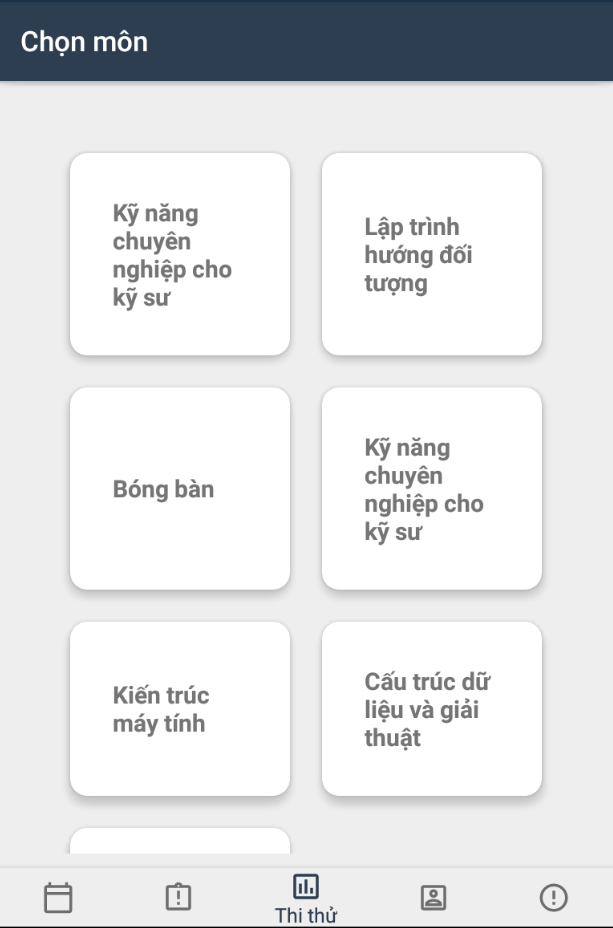
\includegraphics[scale=.3]{select_sub_ui.png}
    \caption{Giao diện màn hình chọn môn thi thử}
    \label{fig:sel_sub}
\end{figure}
Nếu môn học được chọn có dữ liệu câu hỏi trên \textit{Firebase} sẽ hiện ra mã đề thi để chọn. Còn nếu không sẽ thông báo không có dữ liệu. Giả sử là môn học được chọn có dữ liệu câu hỏi, sau khi chọn xong mã đề, lúc này màn hình sẽ hiển thị giao diện thi trắc nghiệm.
\begin{figure}[H]
    \centering
    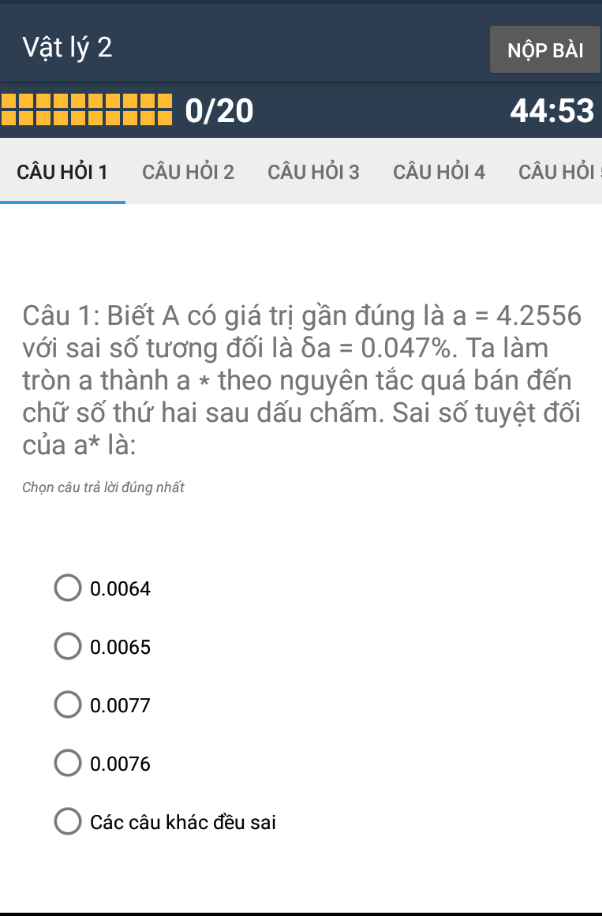
\includegraphics[scale=.3]{ques_ui.png}
    \caption{Giao diện màn hình chọn môn thi thử}

\end{figure}
Chúng ta có thể nộp bài bất cứ khi nào muốn hoặc hết giờ sẽ tự động nộp bài. Sau đó, sẽ hiển thị số câu trả lời đúng, câu trả lời sai có màu đỏ, câu không trả lời có màu vàng, câu trả lời đúng có màu xanh. Chúng ta cũng có thể xem đáp án chi tiết nếu muốn.
\begin{figure}[H]
    \centering
    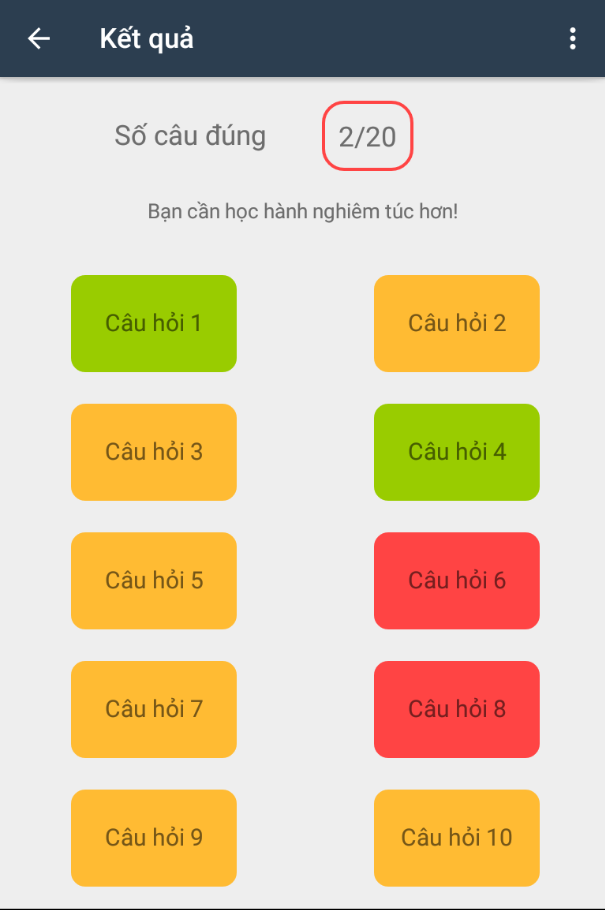
\includegraphics[scale=.3]{mark_ui.png}
    \caption{Giao diện màn hình chọn môn thi thử}

\end{figure}
\begin{figure}[H]
    \centering
    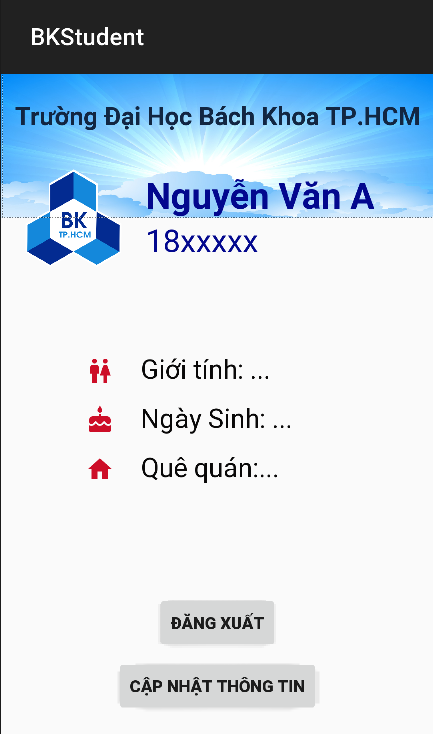
\includegraphics[scale=.4]{info_ui.png}
    \caption{Giao diện màn hình chọn môn thi thử}
    \label{fig:sel_info}
\end{figure}
Giao diện cửa số thông tin cá nhân như ở hình \ref{fig:sel_info}. Chúng ta có thể cập nhật lại thông tin, hoặc đăng xuất tài khoản. Giao diện chức năng cuối cùng như ở hình dưới.
\begin{figure}[H]
    \centering
    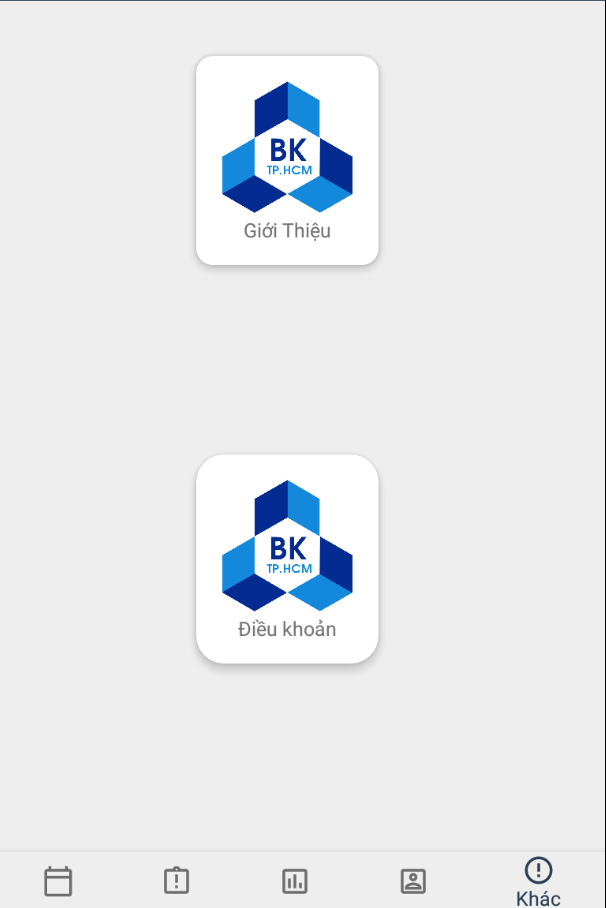
\includegraphics[scale=.4]{other_ui.png}
    \caption{Giao diện màn hình điều khoản, sử dụng}

\end{figure}
\section{Hạn chế}
\begin{itemize}
    \item Ứng dụng còn nhiều hạn chế về chức năng, độ hoàn thiện, giao diện chưa thật sự đẹp.
    \item Ứng dụng còn phụ thuộc vào trang \textit{mybk.hcmut.edu.vn}.
    \item Trải nghiệm chưa thật sự tốt.
\end{itemize}
\newpage
\begin{thebibliography}{}
\bibitem{} Trường đại học Bách Khoa TP. Hồ Chí Minh, logo, \url{https://upload.wikimedia.org/wikipedia/vi/thumb/c/cd/Logo-hcmut.svg/1004px-Logo-hcmut.svg.png}, xem ngày 16/11/2019.
\bibitem{} Trường đại học Bách Khoa TP. Hồ Chí Minh, MyBK, \url{http://mybk.hcmut.edu.vn/}, xem ngày 16/11/2019.
\bibitem{} Google, Material Icons,  \url{https://material.io/resources/icons/?style=baseline}, xem ngày 16/11/2019 
\bibitem{} Google, Firebase, \url{https://firebase.google.com/}, xem ngày 16/11/2019. 
\bibitem{} Frank A. Krueger, SQLite Net, \url{https://github.com/praeclarum/sqlite-net}, xem ngày 16/11/2019
\bibitem{} Ruslan Khuduev, xNet, \url{https://github.com/X-rus/xNet}, xem ngày 16/11/2019.
\bibitem{} Microsoft, Xamarin, \url{https://dotnet.microsoft.com/apps/xamarin}, xem ngày 16/11/2019
\bibitem{} Internet, Midterm image, \url{https://blackmanvoice.net/wp-content/uploads/2017/12/midterm.png}, xem ngày 16/11/2019
\bibitem{} Internet, Finalterm image,\url{https://pbs.twimg.com/profile_images/633646753565143040/y3USaxs3.jpg}, xem ngày 16/11/2019
\end{thebibliography}
\end{document}